\setcounter{ex}{0} 
\subsection{Trắc nghiệm (2 điểm)}
\Opensolutionfile{ans}[ans/ans10] 


%%Câu 1:
\begin{ex}
Cho hệ phương trình
$\begin{cases}
-5x-y=-4\\
-4x-y=-3
\end{cases}$
có nghiệm duy nhất $(x;y)$. Giá trị của biểu thức $-2x^2+3y^2$ là
\choice
{$-9$}
{\True $1$}
{$11$}
{$-4$}
\end{ex}

%%Câu 2:
\begin{ex}
Cho biểu thức
$P=\dfrac{\sqrt{x+4}-2}{x}$ với $x>0$.
Bằng cách trục căn thức ở tử và rút gọn biểu thức $P$, ta được kết quả là
\vspace{0.25cm}
\choice
{$\dfrac{\sqrt{x+4}+2}{x}$}
{$\dfrac{1}{\sqrt{x+4}-2}$}
{\True $\dfrac{1}{\sqrt{x+4}+2}$}
{$\dfrac{1}{\sqrt{x+4}+4}$}
\end{ex}

%%Câu 3:
\begin{ex}
Nếu $a,b$ và $c$ là các số bất kì và $a>b$ thì bất đẳng thức nào sau đây luôn đúng?
\choice
{$ac>bc$}
{$a^2>b^2$}
{$c-a>c-b$}
{\True $a+c>b+c$}
\end{ex}

%%Câu 4:
\begin{ex}
Tập nghiệm của phương trình $\sqrt{2x+3}=x$ là
\choice
{\True $S=\{3\}$}
{$S=\{-1\}$}
{$S=\{-1;3\}$}
{$S=\varnothing$}
\end{ex}

%%Câu 5:
\begin{ex}
Hai hãng taxi có bảng giá như sau:
Hãng A thu phí mở cửa $20\,000$ đồng và $12\,000$ đồng cho mỗi km.
Hãng B thu phí mở cửa $50\,000$ đồng và $8\,000$ đồng cho mỗi km.
Gọi $x$ (km) là quãng đường di chuyển $(x>0)$. Hỏi với điều kiện nào của $x$ thì đi hãng A tiết kiệm hơn hãng B?
\choice
{$x>\dfrac{15}{2}$}
{$x\ge\dfrac{15}{2}$}
{$0<x\le\dfrac{15}{2}$}
{\True $0<x<\dfrac{15}{2}$}
\end{ex}

%%Câu 6:
\begin{ex}
Trong các phương trình sau, phương trình nào là phương trình bậc nhất hai ẩn?
\choice
{$2x^2-y=1$}
{\True $\dfrac{3x}{2}-\dfrac{5}{7}y=1$}
{$\dfrac{5}{3x}-\dfrac{2}{y}=\dfrac{1}{2}$}
{$0x+0y=9$}
\end{ex}

%%Câu 7:
\begin{ex}
Cho hai đường tròn đồng tâm $(O)$ có bán kính lần lượt là $10\,\text{cm}$ và $6\,\text{cm}$. Phần hình vành khuyên nằm trong một góc ở tâm $90^\circ$ có diện tích bằng
\choice
{$25\pi\,\text{cm}^2$}
{$64\pi\,\text{cm}^2$}
{\True $16\pi\,\text{cm}^2$}
{$34\pi\,\text{cm}^2$}
\end{ex}

%%Câu 8:
\begin{ex}
Cho đường tròn $(O)$ và điểm $P$ nằm ngoài đường tròn. Từ $P$ kẻ hai tiếp tuyến $PA$, $PB$ với đường tròn $(O)$ ($A$, $B$ là các tiếp điểm). Biết $\widehat{APB}=70^\circ$. Số đo góc $\widehat{AOB}$ bằng
\choice
{\True $110^\circ$}
{$70^\circ$}
{$140^\circ$}
{$55^\circ$}
\end{ex}

%%Câu 9:
\begin{ex}
Gọi $x$ là số tuổi nam giới. Bất đẳng thức nào biểu diễn điều kiện nam giới phải từ đủ 20 tuổi trở lên để đáp ứng quy định về độ tuổi kết hôn?
\choice
{$x>20$}
{\True $x\ge 20$}
{$x\le 20$}
{$x<20$}
\end{ex}

%%Câu 10:
\begin{ex}
Cho đường tròn $(O;13\,\text{cm})$ có dây cung $AB$ cách tâm $O$ một khoảng bằng $5\,\text{cm}$. Độ dài dây cung $AB$ là
\choice
{$12\,\text{cm}$}
{$\sqrt{194}\,\text{cm}$}
{$26\,\text{cm}$}
{\True $24\,\text{cm}$}
\end{ex}

    
\Closesolutionfile{ans}
\Opensolutionfile{ansbook}[ans/ansbook10]
\setcounter{bt}{0}
\subsection{Tự luận (8 điểm)}

%%Bài 1:

\begin{bt}[1,5 điểm]
Giải các phương trình, bất phương trình và hệ phương trình sau:
\begin{listEX}[3]
\item $(2x-1)^2=9(x-2)^2$
\item $3-\dfrac{2x-5}{4}\le\dfrac{3x+1}{6}-\dfrac{x-2}{3}$
\item $\begin{cases}
\dfrac{3x-y}{4}+\dfrac{x+2y}{3}=\dfrac{1}{6}\\
2(x+1)-3(y-2)=-3
\end{cases}$
\end{listEX}


\loigiai{
\begin{enumerate}
\item Ta có
\begin{align*}
&(2x-1)^2=9(x-2)^2\\
&(2x-1)^2-\big[3(x-2)\big]^2=0\\
&\big[(2x-1)-3(x-2)\big]\big[(2x-1)+3(x-2)\big]=0\\
&(5-x)(5x-7)=0.
\end{align*}
Do đó $x=5$ hoặc $x=\dfrac{7}{5}$.

\item Thu gọn vế phải rồi nhân cả hai vế với $12>0$:
\begin{align*}
3-\dfrac{2x-5}{4}&\le \dfrac{x+5}{6}\\
3(17-2x)&\le 2(x+5)\\
51-6x&\le 2x+10\\
41&\le 8x\\
x&\ge \dfrac{41}{8}.
\end{align*}
Vậy bất phương trình có nghiệm $x\ge\dfrac{41}{8}$.

\item Dùng phương pháp cộng đại số, ta có
\begin{align*}
&\begin{cases}
\dfrac{3x-y}{4}+\dfrac{x+2y}{3}=\dfrac{1}{6},\\
2(x+1)-3(y-2)=-3
\end{cases}\\[0.7em]
\Leftrightarrow\quad
&\begin{cases}
13x+5y=2,\\
2x-3y=-11
\end{cases}\\[0.7em]
\Leftrightarrow\quad
&\begin{cases}
39x+15y=6,\\
10x-15y=-55
\end{cases}\\[0.7em]
\Leftrightarrow\quad
&\begin{cases}
49x=-49,\\
2x-3y=-11
\end{cases}\\[0.7em]
\Leftrightarrow\quad
&\begin{cases}
x=-1,\\
y=3.
\end{cases}
\end{align*}
Vậy hệ phương trình có nghiệm $(x;y)=(-1;3)$.
\end{enumerate}
}
\end{bt}


%%Bài 2:

\begin{bt}[1 điểm]
Rút gọn các biểu thức sau:
\begin{listEX}[1]
\item $A=\sqrt{9x^2-12x+4}+\sqrt{4x^2-20x+25}
-\sqrt{x^2-2x+1}$, với $1\le x\le 2$.

\item $B=\left(\dfrac{2}{\sqrt{x}-1}
-\dfrac{3}{\sqrt{x}+1}\right)
\cdot\dfrac{x-1}{\sqrt{x}+5}$,
với $x\ge 0,\ x\ne 1$.
\end{listEX}
\loigiai{
\begin{enumerate}
\setlength{\itemsep}{1em}

\item Ta có
\begin{align*}
9x^2-12x+4&=(3x-2)^2,\\
4x^2-20x+25&=(2x-5)^2,\\
x^2-2x+1&=(x-1)^2.
\end{align*}
Vì $1\le x\le2$ nên $3x-2>0$, $2x-5<0$ và $x-1\ge0$. Do đó
\begin{align*}
A
&=|3x-2|+|2x-5|-|x-1|\\
&=3x-2+5-2x-(x-1)\\
&=4.
\end{align*}
Vậy $A=4$.

\item Với $x\ge0$ và $x\ne1$, ta có
\begin{align*}
B
&=\left(\dfrac{2}{\sqrt{x}-1}
-\dfrac{3}{\sqrt{x}+1}\right)
\cdot\dfrac{x-1}{\sqrt{x}+5}\\
&=\dfrac{2(\sqrt{x}+1)-3(\sqrt{x}-1)}{x-1}
\cdot\dfrac{x-1}{\sqrt{x}+5}\\
&=\dfrac{5-\sqrt{x}}{x-1}
\cdot\dfrac{x-1}{\sqrt{x}+5}\\
&=\dfrac{5-\sqrt{x}}{\sqrt{x}+5}.
\end{align*}
Vậy $B=\dfrac{5-\sqrt{x}}{\sqrt{x}+5}$.
\end{enumerate}
}
\end{bt}


%%Bài 3:
\begin{bt}[1,0 điểm]
Một hộ gia đình dùng điện theo cách tính: $50$ kWh đầu tiên giá $1\,800$ đồng/kWh, mỗi kWh tiếp theo giá $2\,500$ đồng/kWh. Hộ này dùng nhiều hơn $50$ kWh và muốn tiền điện không vượt quá $350\,000$ đồng. Hỏi hộ dùng được nhiều nhất bao nhiêu kWh? Biết số điện sử dụng là số nguyên.
\loigiai{
Gọi $x$ (kWh) là số điện hộ gia đình sử dụng. Theo giả thiết, $x$ nguyên và $x>50$.

Tiền điện là
\[
1\,800\cdot 50+2\,500(x-50)=90\,000+2\,500x-125\,000=2\,500x-35\,000
\]
(đồng).

Vì tiền điện không vượt quá $350\,000$ đồng nên
\begin{align*}
2\,500x-35\,000&\le 350\,000\\
2\,500x&\le 385\,000\\
x&\le\dfrac{385\,000}{2\,500}\\
x&\le 154.
\end{align*}
Kết hợp $x>50$ và $x$ nguyên, ta được $51\le x\le 154$. Giá trị lớn nhất là $x=154$.

\emph{Kiểm tra.} Với $154$ kWh, số điện vượt $50$ kWh đầu là $104$ kWh. Tiền điện là
\[
1\,800\cdot 50+2\,500\cdot 104=90\,000+260\,000=350\,000
\]
(đồng), đúng bằng mức cho phép. Với $155$ kWh, tiền điện là $352\,500$ đồng, vượt $350\,000$ đồng.

Vậy hộ dùng được nhiều nhất $154$ kWh.
}
\end{bt}

%%Bài 4:
\begin{bt}[1,0 điểm]
Một tấm bìa hình chữ nhật kích thước $20$ cm $\times$ $16$ cm. Người ta cắt bỏ bốn hình vuông bằng nhau, cạnh $x$ cm, ở bốn góc rồi gấp thành một hộp không nắp ($0<x<8$). Phần còn lại ở giữa là mặt đáy của hộp (hình vẽ).
\begin{center}
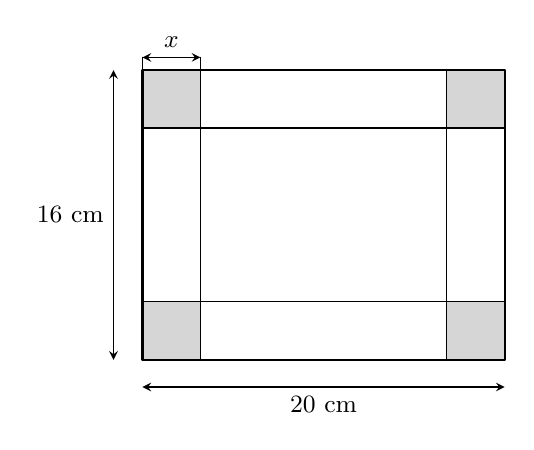
\begin{tikzpicture}[x=0.23cm, y=0.23cm, font=\small, line join=round, line cap=round, >=stealth]
	\fill[gray!32] (0,0) rectangle (3.2,3.2);
	\fill[gray!32] (16.8,0) rectangle (20,3.2);
	\fill[gray!32] (0,12.8) rectangle (3.2,16);
	\fill[gray!32] (16.8,12.8) rectangle (20,16);
	\draw[thick] (0,0) rectangle (20,16);
	\draw (3.2,0)--(3.2,16) (16.8,0)--(16.8,16);
	\draw (0,3.2)--(20,3.2) (0,12.8)--(20,12.8);
	\draw[<->] (0,-1.5)--(20,-1.5) node[midway,below] {$20$ cm};
	\draw[<->] (-1.6,0)--(-1.6,16) node[midway,left] {$16$ cm};
	\draw[<->] (0,16.7)--(3.2,16.7) node[midway,above] {$x$};
	\draw (0,16)--(0,16.7) (3.2,16)--(3.2,16.7);
\end{tikzpicture}
\end{center}
\begin{enumerate}
\item Viết biểu thức diện tích bốn hình vuông bị cắt và diện tích mặt đáy hộp theo $x$.
\item Biết diện tích mặt đáy hộp là $192$ cm$^2$. Tìm $x$.
\end{enumerate}
\loigiai{
\begin{enumerate}
\item Bốn hình vuông bị cắt có tổng diện tích
\[
S_{\text{cắt}}=4x^2\ \text{(cm}^2\text{)}.
\]
Sau khi cắt, mặt đáy có chiều dài $20-2x$ (cm) và chiều rộng $16-2x$ (cm). Diện tích mặt đáy là
\begin{align*}
S_{\text{đáy}}
&=(20-2x)(16-2x)\\
&=4(10-x)(8-x)\\
&=4\bigl(80-18x+x^2\bigr)\\
&=4x^2-72x+320\ \text{(cm}^2\text{)}.
\end{align*}

\item Ta có
\begin{align*}
(20-2x)(16-2x)&=192\\
4(10-x)(8-x)&=192\\
(10-x)(8-x)&=48\\
80-18x+x^2&=48\\
x^2-18x+32&=0\\
(x-16)(x-2)&=0.
\end{align*}
Suy ra $x=16$ hoặc $x=2$.

Vì $0<x<8$ nên $x=16$ bị loại. Với $x=2$, mặt đáy có kích thước $16$ cm và $12$ cm.

\emph{Kiểm tra.} Diện tích mặt đáy là $16\cdot 12=192$ (cm$^2$).

Vậy $x=2$ cm.
\end{enumerate}
}
\end{bt}

%%Bài 5:
\begin{bt}[1,0 điểm]
Một vòi phun nước tưới một vùng đất hình quạt tròn tâm $O$, góc ở tâm $\widehat{AOB}=120^\circ$. Độ dài cung $AB$ là $8\pi$ m (hình vẽ).
\begin{center}
\begin{tikzpicture}[scale=1.15, font=\small, line join=round, line cap=round]
	\coordinate (O) at (0,0);
	\coordinate (A) at (0:3);
	\coordinate (B) at (120:3);
	\fill[blue!8] (O)--(A) arc (0:120:3) -- cycle;
	\draw[thick] (O)--(A) arc (0:120:3) -- cycle;
	\pic[draw, angle radius=0.85cm, angle eccentricity=1.45] {angle = A--O--B};
	\node at (60:1.45) {$120^\circ$};
	\node at (60:3.45) {$8\pi$ m};
	\fill (O) circle (1.1pt) node[below] {$O$};
	\fill (A) circle (1.1pt) node[right] {$A$};
	\fill (B) circle (1.1pt) node[above left] {$B$};
\end{tikzpicture}
\end{center}
\begin{enumerate}
\item Tính bán kính của vùng đất được tưới.
\item Tính diện tích vùng đất được tưới.
\end{enumerate}
\loigiai{
\begin{enumerate}
\item Gọi $R$ (m) là bán kính vùng đất, $R>0$. Độ dài cung $AB$ chắn góc ở tâm $120^\circ$ là
\begin{align*}
\dfrac{\pi R\cdot 120}{180}&=8\pi\\
\dfrac{2R}{3}&=8\\
R&=12.
\end{align*}
Vậy bán kính vùng đất được tưới là $12$ m.

\item Diện tích hình quạt bán kính $12$ m, góc ở tâm $120^\circ$, là
\begin{align*}
S
&=\dfrac{\pi R^2 n}{360}\\
&=\dfrac{\pi\cdot 12^2\cdot 120}{360}\\
&=\dfrac{\pi\cdot 144}{3}\\
&=48\pi\ \text{(m}^2\text{)}.
\end{align*}
Vậy diện tích vùng đất được tưới là $48\pi$ m$^2$.
\end{enumerate}
}
\end{bt}

%%Bài 6:
\begin{bt}[0,5 điểm]
Giải bất phương trình sau: 
\[\dfrac{x+2021}{2022}+\dfrac{x+2022}{2023}<\dfrac{x+2023}{2024}+\dfrac{x+2024}{2025}\]
\loigiai{
$x=1$

Gợi ý: cộng hai vế của phương trình với -2: 
\[\dfrac{x-1}{2022}+\dfrac{x-1}{2023}>\dfrac{x-1}{2024}+\dfrac{x-1}{2025}\]
}
\end{bt}

\Closesolutionfile{ansbook}
